\documentclass[]{article}
\usepackage{lmodern}
\usepackage{amssymb,amsmath}
\usepackage{ifxetex,ifluatex}
\usepackage{fixltx2e} % provides \textsubscript
\ifnum 0\ifxetex 1\fi\ifluatex 1\fi=0 % if pdftex
  \usepackage[T1]{fontenc}
  \usepackage[utf8]{inputenc}
\else % if luatex or xelatex
  \ifxetex
    \usepackage{mathspec}
  \else
    \usepackage{fontspec}
  \fi
  \defaultfontfeatures{Ligatures=TeX,Scale=MatchLowercase}
\fi
% use upquote if available, for straight quotes in verbatim environments
\IfFileExists{upquote.sty}{\usepackage{upquote}}{}
% use microtype if available
\IfFileExists{microtype.sty}{%
\usepackage{microtype}
\UseMicrotypeSet[protrusion]{basicmath} % disable protrusion for tt fonts
}{}
\usepackage[margin=1in]{geometry}
\usepackage{hyperref}
\hypersetup{unicode=true,
            pdftitle={Trabajo Práctico Final Biometría II - 2021},
            pdfauthor={Matías Alemán, Milagros Azcueta, Manuel Fiz, Emilia Haberfeld, Diego Kafer, Ilán Shalom},
            pdfborder={0 0 0},
            breaklinks=true}
\urlstyle{same}  % don't use monospace font for urls
\usepackage{color}
\usepackage{fancyvrb}
\newcommand{\VerbBar}{|}
\newcommand{\VERB}{\Verb[commandchars=\\\{\}]}
\DefineVerbatimEnvironment{Highlighting}{Verbatim}{commandchars=\\\{\}}
% Add ',fontsize=\small' for more characters per line
\usepackage{framed}
\definecolor{shadecolor}{RGB}{248,248,248}
\newenvironment{Shaded}{\begin{snugshade}}{\end{snugshade}}
\newcommand{\AlertTok}[1]{\textcolor[rgb]{0.94,0.16,0.16}{#1}}
\newcommand{\AnnotationTok}[1]{\textcolor[rgb]{0.56,0.35,0.01}{\textbf{\textit{#1}}}}
\newcommand{\AttributeTok}[1]{\textcolor[rgb]{0.77,0.63,0.00}{#1}}
\newcommand{\BaseNTok}[1]{\textcolor[rgb]{0.00,0.00,0.81}{#1}}
\newcommand{\BuiltInTok}[1]{#1}
\newcommand{\CharTok}[1]{\textcolor[rgb]{0.31,0.60,0.02}{#1}}
\newcommand{\CommentTok}[1]{\textcolor[rgb]{0.56,0.35,0.01}{\textit{#1}}}
\newcommand{\CommentVarTok}[1]{\textcolor[rgb]{0.56,0.35,0.01}{\textbf{\textit{#1}}}}
\newcommand{\ConstantTok}[1]{\textcolor[rgb]{0.00,0.00,0.00}{#1}}
\newcommand{\ControlFlowTok}[1]{\textcolor[rgb]{0.13,0.29,0.53}{\textbf{#1}}}
\newcommand{\DataTypeTok}[1]{\textcolor[rgb]{0.13,0.29,0.53}{#1}}
\newcommand{\DecValTok}[1]{\textcolor[rgb]{0.00,0.00,0.81}{#1}}
\newcommand{\DocumentationTok}[1]{\textcolor[rgb]{0.56,0.35,0.01}{\textbf{\textit{#1}}}}
\newcommand{\ErrorTok}[1]{\textcolor[rgb]{0.64,0.00,0.00}{\textbf{#1}}}
\newcommand{\ExtensionTok}[1]{#1}
\newcommand{\FloatTok}[1]{\textcolor[rgb]{0.00,0.00,0.81}{#1}}
\newcommand{\FunctionTok}[1]{\textcolor[rgb]{0.00,0.00,0.00}{#1}}
\newcommand{\ImportTok}[1]{#1}
\newcommand{\InformationTok}[1]{\textcolor[rgb]{0.56,0.35,0.01}{\textbf{\textit{#1}}}}
\newcommand{\KeywordTok}[1]{\textcolor[rgb]{0.13,0.29,0.53}{\textbf{#1}}}
\newcommand{\NormalTok}[1]{#1}
\newcommand{\OperatorTok}[1]{\textcolor[rgb]{0.81,0.36,0.00}{\textbf{#1}}}
\newcommand{\OtherTok}[1]{\textcolor[rgb]{0.56,0.35,0.01}{#1}}
\newcommand{\PreprocessorTok}[1]{\textcolor[rgb]{0.56,0.35,0.01}{\textit{#1}}}
\newcommand{\RegionMarkerTok}[1]{#1}
\newcommand{\SpecialCharTok}[1]{\textcolor[rgb]{0.00,0.00,0.00}{#1}}
\newcommand{\SpecialStringTok}[1]{\textcolor[rgb]{0.31,0.60,0.02}{#1}}
\newcommand{\StringTok}[1]{\textcolor[rgb]{0.31,0.60,0.02}{#1}}
\newcommand{\VariableTok}[1]{\textcolor[rgb]{0.00,0.00,0.00}{#1}}
\newcommand{\VerbatimStringTok}[1]{\textcolor[rgb]{0.31,0.60,0.02}{#1}}
\newcommand{\WarningTok}[1]{\textcolor[rgb]{0.56,0.35,0.01}{\textbf{\textit{#1}}}}
\usepackage{graphicx}
% grffile has become a legacy package: https://ctan.org/pkg/grffile
\IfFileExists{grffile.sty}{%
\usepackage{grffile}
}{}
\makeatletter
\def\maxwidth{\ifdim\Gin@nat@width>\linewidth\linewidth\else\Gin@nat@width\fi}
\def\maxheight{\ifdim\Gin@nat@height>\textheight\textheight\else\Gin@nat@height\fi}
\makeatother
% Scale images if necessary, so that they will not overflow the page
% margins by default, and it is still possible to overwrite the defaults
% using explicit options in \includegraphics[width, height, ...]{}
\setkeys{Gin}{width=\maxwidth,height=\maxheight,keepaspectratio}
\IfFileExists{parskip.sty}{%
\usepackage{parskip}
}{% else
\setlength{\parindent}{0pt}
\setlength{\parskip}{6pt plus 2pt minus 1pt}
}
\setlength{\emergencystretch}{3em}  % prevent overfull lines
\providecommand{\tightlist}{%
  \setlength{\itemsep}{0pt}\setlength{\parskip}{0pt}}
\setcounter{secnumdepth}{0}
% Redefines (sub)paragraphs to behave more like sections
\ifx\paragraph\undefined\else
\let\oldparagraph\paragraph
\renewcommand{\paragraph}[1]{\oldparagraph{#1}\mbox{}}
\fi
\ifx\subparagraph\undefined\else
\let\oldsubparagraph\subparagraph
\renewcommand{\subparagraph}[1]{\oldsubparagraph{#1}\mbox{}}
\fi

%%% Use protect on footnotes to avoid problems with footnotes in titles
\let\rmarkdownfootnote\footnote%
\def\footnote{\protect\rmarkdownfootnote}

%%% Change title format to be more compact
\usepackage{titling}

% Create subtitle command for use in maketitle
\providecommand{\subtitle}[1]{
  \posttitle{
    \begin{center}\large#1\end{center}
    }
}

\setlength{\droptitle}{-2em}

  \title{Trabajo Práctico Final\\
Biometría II - 2021}
    \pretitle{\vspace{\droptitle}\centering\huge}
  \posttitle{\par}
    \author{Matías Alemán, Milagros Azcueta, Manuel Fiz, Emilia Haberfeld, Diego
Kafer, Ilán Shalom}
    \preauthor{\centering\large\emph}
  \postauthor{\par}
      \predate{\centering\large\emph}
  \postdate{\par}
    \date{16/11/2021}


\begin{document}
\maketitle

\hypertarget{introducciuxf3n}{%
\section{Introducción}\label{introducciuxf3n}}

Los animales se encuentran constantemente tomando decisiones respecto a
cuándo alimentarse, aparearse, dormir, y demás acciones (1). A través de
aprendizajes y experiencias previas, son capaces de comparar dos o más
escenarios probables antes de realizar cualquier acción (2). La
generación de una expectativa respecto a dichos escenarios es un proceso
que permite a los animales predecir la aparición de estímulos (tanto
aversivos como apetitivos) y de este modo, adaptar su comportamiento
(3). Esta expectativa incide directamente en sus capacidades mnésicas,
debido a que el aprendizaje depende de asociaciones entre claves
externas y representaciones internas de dichas claves (4). Este proceso
ha sido ampliamente estudiado en vertebrados, pero hay menos información
disponible en invertebrados.

El objetivo de este trabajo es estudiar la modulación de memorias a
largo término a partir de cambios en la expectativa de la recompensa. El
modelo experimental es la abeja Apis mellifera y los experimentos fueron
realizados en un contexto controlado dentro del laboratorio.

\hypertarget{materiales-y-muxe9todos}{%
\section{Materiales y métodos}\label{materiales-y-muxe9todos}}

Abejas Apis mellifera fueron entrenadas bajo un condicionamiento clásico
del reflejo de extensión de probóscide (de aquí en más PER, por sus
siglas en inglés) (5,6): se administra un odorante a la vez que se tocan
las antenas con una gota de sacarosa. La abeja extiende su probóscide
como reflejo de este estímulo, y en ese momento se la alimenta con una
solución azucarada. De este entrenamiento, recibieron 4 ensayos.
Terminada la etapa de entrenamiento, se realizaron tres testeos donde se
presentó solo el odorante a 3, 24 y 48 hs posteriores al último ensayo
de entrenamiento.

Las abejas se dividieron en 4 grupos experimentales dependiendo de la
sacarosa recibida en las antenas y en la probóscide. Los grupos
``constante alto'' y ``constante bajo'' recibieron tanto en las antenas
como en la probóscide azúcar de concentración 1,5 M y 0,5 M
respectivamente. Por otro lado, los grupos ``contraste positivo'' y
``contraste negativo'' recibieron azúcar de distinta concentración en
cada pieza sensorial: los animales del grupo contraste positivo
recibieron sacarosa 0,5 M en las antenas y 1,5 M en su probóscide. Por
otro lado, los animales del contraste negativo recibieron azúcar 1,5 M
en las antenas para luego ser alimentados con sacarosa 0,5 M.

A continuación se presentan gráficos en base a una estadística
descriptiva exploratoria para observar la tendencia de los datos:

\begin{Shaded}
\begin{Highlighting}[]
\NormalTok{gp_entr   }\CommentTok{# Grafico de perfiles de la etapa de entrenamiento}
\end{Highlighting}
\end{Shaded}

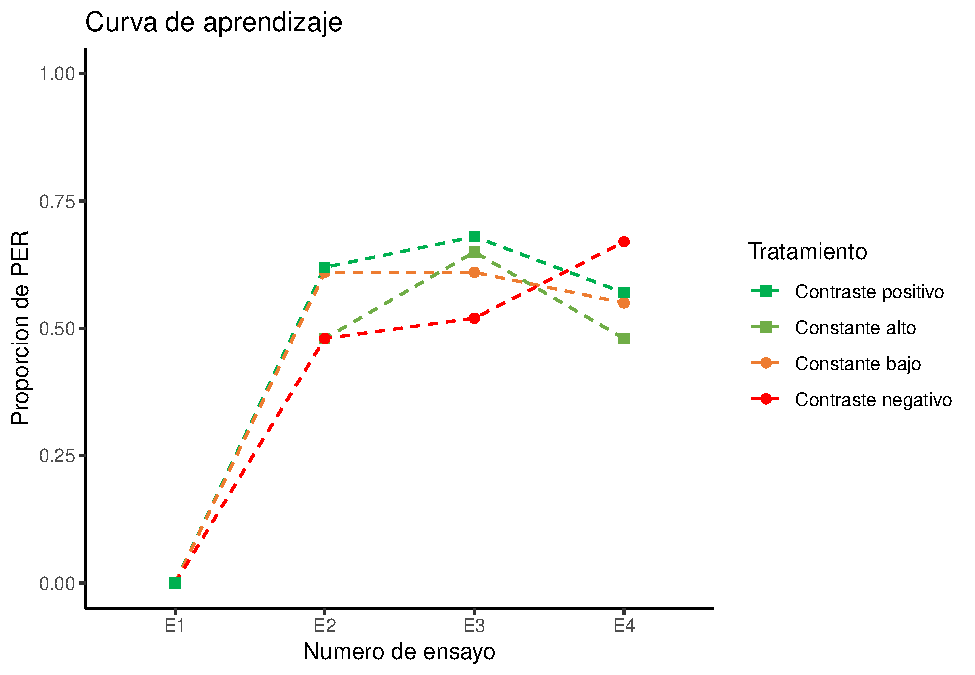
\includegraphics{TP_FINAL_RMarkdown_files/figure-latex/unnamed-chunk-3-1.pdf}
\textbf{Figura 1:} Proporciones de PER para cada tratamiento en cada
ensayo de entrenamiento. En la etapa de entrenamiento, se observa que
todos los animales parten de una respuesta nula al odorante en el ensayo
1. En los ensayos subsiguientes todos los grupos parecen alcanzar una
proporción de PER asintótica alrededor de 0,6, lo que se traduce en un
buen aprendizaje de la asociación odorante-recompensa.

\begin{Shaded}
\begin{Highlighting}[]
\NormalTok{gp_testeo }\CommentTok{# Grafico de perfiles de la etapa de evaluacion}
\end{Highlighting}
\end{Shaded}

\includegraphics{TP_FINAL_RMarkdown_files/figure-latex/unnamed-chunk-4-1.pdf}
\textbf{Figura 2:} Proporciones de PER para cada tratamiento en cada
tiempo de evaluación. Respecto a la etapa de evaluación, a 3 hs los
resultados parecen ser opuestos a la hipótesis (los grupos CONSTANTE
BAJO y CONTRASTE NEGATIVO tienen respuestas más altas que CONSTANTE ALTO
y CONTRASTE POSITIVO), pero luego, esta relación se revierte en las
pruebas a 24 y 48 hs.

\begin{Shaded}
\begin{Highlighting}[]
\NormalTok{gp_semana }\CommentTok{# Grafico de perfiles de la etapa de evaluacion por semana}
\end{Highlighting}
\end{Shaded}

\includegraphics{TP_FINAL_RMarkdown_files/figure-latex/unnamed-chunk-5-1.pdf}
\textbf{Figura 3:} Respecto a la proporción de PER en cada tiempo de
evaluación en cada semana, se observa cierto grado de variabilidad en
las respuestas. Resulta conveniente incluirla como variable explicatoria
del modelo.

\hypertarget{modelado}{%
\section{Modelado}\label{modelado}}

Como VR se midió la extensión de la probóscide frente al olor (si-no).
Al ser una variable dicotómica, la distribución de probabilidades
esperada es una Bernoulli. El diseño es de medidas repetidas ya que cada
abeja fue medida 7 veces (4 ensayos de entrenamiento + 3 testeos). Se
realizó estadística descriptiva de la etapa de entrenamiento y un modelo
estadístico para la etapa de evaluación ya que el mayor interés del
análisis está depositado en las diferencias observables durante esta
etapa. Como variables explicativas se incluyeron:

VE1: Tiempo de testeo → cualitativa fija de 3 niveles (3, 24, 48 hs).

VE2: Tratamiento → cualitativa fija de 4 niveles (constante alto,
constante bajo, contraste positivo, contraste negativo)

VE3: ID de abeja → cualitativa aleatoria de 132 niveles (abeja 1 a 132).

VE4: Semana de trabajo → cualitativa aleatoria de 7 niveles (semanas 1 a
7). Covariable.

Se implementó un modelo lineal generalizado condicional con la función
glmmTMB de la librería glmmTMB. Se optó por un modelo condicional ya que
se compararon modelos marginales con distintas matrices de correlación
y, a partir de un ranking de QIC (el cual compara modelos según su
verosimilitud y cantidad de parámetros estimados), el más conveniente
resultó ser un modelo marginal con matriz de simetría compuesta. Como
los modelos condicionales tienen implícita una matriz de simetría
compuesta y resultan más familiares para su implementación en R, se
elige esta opción. Desde un punto de vista más teórico quisimos, en un
principio, incluir a la variable ``semana'' como una de efectos
aleatorios, dado que no presentamos preguntas o hipótesis puntuales
acerca de las diferencias entre semanas. Sin embargo, al chequear los
supuestos, el supuesto de normalidad de los residuos de la variable de
efectos aleatorios ``ID'' no cumplía las expectativas.

Como solución a este problema decidimos probar incluir en el modelo la
variable semana como una de efectos fijos. El modelo ahora incluye más
parámetros y por lo tanto logra un mejor ajuste, resultando en predichos
más precisos con nuestros datos. Es por esto que al chequear nuevamente
los supuestos, se logra obtener una prueba satisfactoria de Shapiro-Wilk
para los residuos de la variable de efectos aleatorios ``ID''.

\hypertarget{modelo-teuxf3rico}{%
\subsection{Modelo teórico}\label{modelo-teuxf3rico}}

logit(\[\pi_{ijkl}\]) = \[\mu\] + \[\alpha_i\] + \[\beta_j\] +
\[\alpha*\beta_{ij}\] + \[\gamma_k\] + \[A_{l(ij)(k)}\]

\hypertarget{modelo-implementado-en-r}{%
\subsection{Modelo implementado en R}\label{modelo-implementado-en-r}}

\begin{Shaded}
\begin{Highlighting}[]
\NormalTok{m10 <-}\StringTok{ }\KeywordTok{glmmTMB}\NormalTok{(rta }\OperatorTok{~}\StringTok{ }\NormalTok{TRATAMIENTO}\OperatorTok{*}\NormalTok{tiempo_testeo }\OperatorTok{+}\StringTok{ }\NormalTok{SEMANA }\OperatorTok{+}\StringTok{ }\NormalTok{(}\DecValTok{1}\OperatorTok{|}\NormalTok{ID), }\DataTypeTok{data=}\NormalTok{long_testeo, }\DataTypeTok{family=}\StringTok{"binomial"}\NormalTok{)   }\CommentTok{# Modelo seleccionado: semana como VE de efectos fijos}

\KeywordTok{Anova}\NormalTok{(m10)   }\CommentTok{# Prueba de ANOVA del modelo seleccionado}
\end{Highlighting}
\end{Shaded}

\begin{verbatim}
## Analysis of Deviance Table (Type II Wald chisquare tests)
## 
## Response: rta
##                             Chisq Df Pr(>Chisq)    
## TRATAMIENTO                3.3627  3  0.3390115    
## tiempo_testeo              2.0484  2  0.3590747    
## SEMANA                    24.8214  6  0.0003684 ***
## TRATAMIENTO:tiempo_testeo 26.5204  6  0.0001780 ***
## ---
## Signif. codes:  0 '***' 0.001 '**' 0.01 '*' 0.05 '.' 0.1 ' ' 1
\end{verbatim}

La interacción tratamiento*tiempo resulta significativa. Por ende, no es
posible evaluar efectos principales. Las comparaciones se realizaron con
contrastes ortogonales ya que se poseen hipótesis a priori sobre las
mismas.

\hypertarget{contrastes-a-priori}{%
\subsection{Contrastes a priori}\label{contrastes-a-priori}}

Se espera que el grupo CONTRASTE POSITIVO aprenda la asociación
olor-azúcar más fuertemente que el CONSTANTE ALTO, debido a un mayor
estado motivacional gracias a la ``sorpresa'' recibida en la probóscide
(azúcar 1,5 M) en contraste con el azúcar esperada que tocó las antenas
segundos antes (0,5 M). Caso opuesto, se espera que la proporción de
animales del grupo CONTRASTE NEGATIVO que aprendan la asociación sea
menor que la proporción de animales del grupo CONSTANTE BAJO, debido a
un estado motivacional degradado por la ``decepción'' de recibir azúcar
0,5 M cuando esperaban 1,5 M.

Las comparaciones se realizaron entre grupos con igual concentración de
azúcar en probóscide, dado que la ingesta de alimento, la recompensa, es
la señal post-ingestiva que permite la consolidación de la memoria
asociatva de largo término.

\hypertarget{resultados}{%
\section{Resultados}\label{resultados}}

\begin{Shaded}
\begin{Highlighting}[]
\NormalTok{ortogonales }\CommentTok{# Implementacion de contrastes ortogonales}
\end{Highlighting}
\end{Shaded}

\begin{verbatim}
## $emmeans
##  TRATAMIENTO    tiempo_testeo   prob     SE  df lower.CL upper.CL null t.ratio
##  constante_alto 3hs           0.3916 0.1441 377   0.1638    0.679  0.5  -0.728
##  constante_bajo 3hs           0.7430 0.1193 377   0.4583    0.908  0.5   1.699
##  contraste_neg  3hs           0.7648 0.1097 377   0.4950    0.915  0.5   1.934
##  contraste_pos  3hs           0.4877 0.1379 377   0.2433    0.738  0.5  -0.090
##  constante_alto 24hs          0.3916 0.1441 377   0.1638    0.679  0.5  -0.728
##  constante_bajo 24hs          0.5241 0.1504 377   0.2519    0.783  0.5   0.160
##  contraste_neg  24hs          0.3176 0.1248 377   0.1304    0.591  0.5  -1.328
##  contraste_pos  24hs          0.8030 0.0954 377   0.5545    0.930  0.5   2.329
##  constante_alto 48hs          0.5070 0.1506 377   0.2393    0.771  0.5   0.047
##  constante_bajo 48hs          0.3493 0.1393 377   0.1386    0.642  0.5  -1.015
##  contraste_neg  48hs          0.0642 0.0423 377   0.0168    0.215  0.5  -3.802
##  contraste_pos  48hs          0.8030 0.0954 377   0.5545    0.930  0.5   2.329
##  p.value
##   0.4671
##   0.0902
##   0.0539
##   0.9287
##   0.4671
##   0.8727
##   0.1851
##   0.0204
##   0.9627
##   0.3108
##   0.0002
##   0.0204
## 
## Results are averaged over the levels of: SEMANA 
## Confidence level used: 0.95 
## Intervals are back-transformed from the logit scale 
## Tests are performed on the logit scale 
## 
## $contrasts
##  contrast      odds.ratio    SE  df lower.CL upper.CL null t.ratio p.value
##  3hs_alto_pos       0.676 0.545 377   0.1387    3.297    1  -0.485  0.6277
##  3hs_bajo_neg       0.889 0.767 377   0.1631    4.845    1  -0.137  0.8914
##  24hs_alto_pos      0.158 0.134 377   0.0296    0.842    1  -2.168  0.0308
##  24hs_bajo_neg      2.367 1.980 377   0.4566   12.266    1   1.029  0.3039
##  48hs_alto_pos      0.252 0.213 377   0.0481    1.324    1  -1.634  0.1031
##  48hs_bajo_neg      7.832 7.238 377   1.2726   48.202    1   2.227  0.0265
## 
## Results are averaged over the levels of: SEMANA 
## Confidence level used: 0.95 
## Intervals are back-transformed from the log odds ratio scale 
## Tests are performed on the log odds ratio scale
\end{verbatim}

\begin{Shaded}
\begin{Highlighting}[]
\NormalTok{gp_final  }\CommentTok{# Gráfico final, medidas resumen del modelo}
\end{Highlighting}
\end{Shaded}

\includegraphics{TP_FINAL_RMarkdown_files/figure-latex/unnamed-chunk-11-1.pdf}
\textbf{Figura 4:} Proporciones estimadas de PER para cada tratamiento
en cada tiempo de evaluación. Los resultados se informan como la media
+/- el error estándar de cada combinación de tiempo y tratamiento. A
partir de un modelo mixto/condicional, se vio que la proporción de PER a
24 hs es mayor para el grupo CONTRASTE POSITIVO que para el grupo
CONSTANTE ALTO (p\textless{}0.05) y que la proporción de PER a 48 hs es
menor para el grupo CONTRASTE NEGATIVO que para el grupo CONSTANTE BAJO
(p\textless{}0.05).

En el primer tiempo de evaluación (3 hs) no se observaron diferencias
significativas en los contrastes (p\textgreater{}0,05).

A 24 hs se observaron diferencias significativas entre los grupos
CONSTANTE ALTO y CONTRASTE POSITIVO. Se estima que la chance de
extensión de probóscide para el grupo CONTRASTE POSITIVO aumenta en
promedio entre un 2,96\% y un 84,2\% respecto al grupo CONSTANTE ALTO,
con un 95\% de confianza (p\textless{}0,05). No se observaron
diferencias significativas en la comparación CONSTANTE BAJO vs CONTRASTE
NEGATIVO a 24 hs (p\textgreater{}0,05).

En la evaluación a 48 hs, se observaron diferencias significativas entre
los grupos CONSTANTE BAJO y CONTRASTE NEGATIVO. Se estima que la chance
de extensión de probóscide para el grupo CONTRASTE NEGATIVO disminuye en
promedio entre un 21,4\% y un 97,93\% respecto al grupo CONSTANTE BAJO,
con un 95\% de confianza (p\textless{}0,05). No se observaron
diferencias significativas en la comparación CONSTANTE ALTO vs CONTRASTE
POSITIVO a 48 hs (p\textgreater{}0,05), aunque la tendencia de las
estimaciones coincide con lo observado a 24 hs.

\hypertarget{discusiuxf3n}{%
\section{Discusión}\label{discusiuxf3n}}

Debido a que la interacción tratamiento*tiempo resultó significativa, se
realizaron contrastes ortogonales teniendo en cuenta ambas variables. Si
nos situamos en primer lugar en las comparaciones en t = 3 hs, se
observa que ninguno de los dos contrastes propuestos mostró diferencias
significativas. Lo que es más curioso aun es que la tendencia de la
respuesta parece ser opuesta a la esperada por los contrastes a priori:
los grupos contraste negativo y constante bajo son aquellos que mayor
proporción de PER presentaron. Debido a que la memoria observada a las 3
hs posteriores de finalizado el último ensayo de entrenamiento es una
memoria de corto término, puede estar influida por diversos fenómenos
ajenos al tratamiento aplicado. En particular, se propone que en este
punto temporal hay un conflicto en relación a la expresión de la memoria
generada. Los animales de los grupos contraste negativo y constante bajo
son los que menos azúcar ingirieron (en términos nutricionales), ya que
siempre consumieron azúcar de concentración 0,5 M. Por lo tanto, es muy
probable que a 3 hs estos animales estén más motivados que los otros dos
grupos y que por ende, lo que parece ser una mayor retención de la
memoria (que solo es posible de observar a través de la extensión de la
probóscide, en este experimento) sea un reflejo de la motivación de
estos animales por seguir ingiriendo azúcar. En contraste, las abejas de
los grupos contraste positivo y constante alto habrían alcanzado un
nivel de saciedad más alto, respondiendo menos al estímulo (odorante).

El día siguiente al aprendizaje, se buscó estudiar la consolidación de
memoria de largo término en las abejas. Al hacer las comparaciones a t =
24 hs se observaron diferencias significativas entre los grupos
constante alto y contraste positivo. Esto sugiere que un mismatch
positivo entre lo que el animal capta con las antenas y lo que ingiere
genera una consolidación de memoria de largo término más robusta, la
cual tiene un efecto directo en el comportamiento. Creemos que el animal
al sensar con las antenas genera expectativas de lo que va a ingerir y
es la sorpresa positiva que siente lo que generaría un estado
motivacional que predispone a una mayor retención de la experiencia. Por
otro lado, al comparar constante bajo con contraste negativo no
observamos diferencias significativas. Sin embargo se pudo observar una
tendencia que encaja con lo teorizado a priori: aquellos animales
pertenecientes al grupo contraste negativo presentaron una menor
proporción de PER que el grupo constante bajo. Esto sugiere que puede
haber un efecto en la consolidación de la memoria de largo término por
mismatch negativo.

En la evaluación a 48 hs no se observaron diferencias significativas
entre los grupos constante alto y contraste positivo. Esto puede
explicarse en base a la distribución de probabilidades de nuestros
datos. En una distribución Bernoulli, el punto de máxima varianza se
encuentra en p=0,5. Trasladado al ejemplo de este trabajo, sería el caso
en el cual el 50\% de las abejas extiende su probóscide y el 50\% no lo
hace, bajo un mismo tratamiento. Debido a que la proporción de PER
estimada para el grupo CONSTANTE ALTO a 48 hs es de 0,51, este grupo
tiene la máxima varianza posible. Por lo tanto, a pesar de que se
mantiene la misma tendencia observada en la evaluación a las 24 hs, la
comparación con el grupo CONTRASTE POSITIVO resulta no significativa en
este caso. Por otro lado, la comparación entre los grupos CONSTANTE BAJO
y CONTRASTE NEGATIVO resultó significativa. Se pudo observar que la
sorpresa negativa que sufre el animal en este último grupo es capaz de
modular la memoria a largo término. Si bien la memoria del grupo
constante bajo decae en el tiempo, la memoria del grupo contraste
negativo lo hace a un ritmo mayor.

Como conclusión, resulta interesante haber observado que no solo es
importante que haya un mismatch entre lo esperado y lo obtenido para
modular una memoria a largo término, sino que también la valencia de ese
contraste tendrá un efecto diferencial sobre esa memoria.

\hypertarget{bibliografuxeda}{%
\section{Bibliografía}\label{bibliografuxeda}}

\begin{enumerate}
\def\labelenumi{\arabic{enumi}.}
\tightlist
\item
  McFarland, D. J. Decision making in animals. Nature 269, 15--21
  (1977).
\item
  Menzel, R. \& Giurfa, M. Dimensions of Cognition in an Insect, the
  Honeybee. Behav. Cogn. Neurosci. Rev.~5, 24--40 (2006).
\item
  Gil, M., De Marco, R. J. \& Menzel, R. Learning reward expectations in
  honeybees. Learn. Mem. 14, 491--6 (2007).
\item
  Rescorla, R. A. A Pavlovian analysis of goal-directed behavior. Am.
  Psychol. 42, 119--129 (1987).
\item
  Bitterman, M. E., Menzel, R., Fietz, A. \& Schäfer, S. Classical
  conditioning of proboscis extension in honeybees (Apis mellifera). J.
  Comp. Psychol. 97, 107--119 (1983).
\item
  Takeda, K. Classical conditioned response in the honey bee. J. Insect
  Physiol. 6, 168--179 (1961).
\end{enumerate}


\end{document}
